\clearpage\begingroup\SourceLeaf{98b}\HistoricalHead{93}{R}{GAUSS AN ENCKE.}
\begin{center}[13.]\end{center}
\begin{center}\textsc{Gauss} an \textsc{Encke}.\quad Göttingen, 14. September 1834.\end{center}
\noindent .\ .\ .\ .\ .\ .\ .\ .\ .\ .\ .\ .\ .\ .\ .\ .\ .\ .\ .\ .\ .
\par\noindent\hspace*{\parindent}Es sind schon mehreremale durch meinen Sohn und Dr. \textsc{Goldschmidt}
gleichzeitige Beobachtungen in der Sternwarte und dem M[agnetischen] O[bservatorium]
gemacht, die eine bewundernswürdige Uebereinstimmung geben,
selbst in den Zehnteln der Scalentheile. Versuchsweise wurden dadurch einmahl
die Uhren verglichen, und obwohl durchaus keine grösseren Anomalien
der magn[etischen] Decl[ination] dabei Statt gefunden hatten, fand sich doch
das Resultat bei hinterdrein gemachter Vergleichung durch den Chronometer
auf wenige Zeitsecunden richtig. Also eine neue Methode der Längenbestimmung.

Es sind hier bereits einige Versuche mit den Beobachtungen gemacht,
wo ein 4 {\fontspec{FreeSerif.otf}℔}diger Stab durch ein kleines an einem Ende aufgelegtes Gewicht
horizontal gemacht wurde und nachher, nach Umkehrung der Pole, am andern
Ende. Also die \textsc{Coulombsche} Methode, unter Anwendung des Princips, die
Horizontalstellung durch Spiegel, Scale und Fernrohr zu ermitteln.

Das Fernrohr in der oberen Etage, die Scale an der Decke. Eine vollständige
Beschreibung würde für einen Brief zu weitläuftig sein, und die Entwicklung
mehrerer dabei zu berücksichtigenden Momente erfordern. Aber
einige Idee wird umstehende Figur geben. Dieser Versuch ist gar nicht in
der Absicht gemacht, die Inclination selbst zu bestimmen, da das Local im
phys. Cabinet dazu gar nicht taugt, indem Eisen und andere Magnetstäbe in
\clearpage\SourceLeaf{99a}\HistoricalHead{94}{L}{PHYSIK. BRIEFWECHSEL.}
\noindent der Nähe waren, daher ich auch das Resultat noch gar nicht berechnet habe,
\par\noindent\begin{minipage}[t]{.29\linewidth}\vspace{0pt}\centering
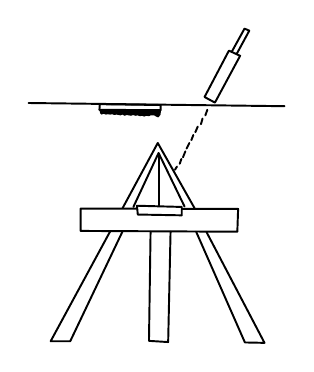
\begin{tikzpicture}[x=.002in,y=-.002in,line width=.7pt,line cap=round,line join=round]
\draw (35,210)--(675,218);
\draw (213,213)--(365,215)--(365,228)--(212,227)--cycle;
\fill (212,227)--(366,228)--(365,239)--(362,243)--(359,246)
 --(354,244)--(349,241)--(340,241)--(336,243)--(329,242)
 --(324,244)--(319,242)--(313,243)--(308,241)--(302,242)
 --(296,240)--(291,242)--(286,241)--(280,240)--(275,242)
 --(269,239)--(265,241)--(260,240)--(255,239)--(249,240)
 --(244,238)--(239,239)--(233,238)--(228,239)--(223,237)
 --(217,239)--(214,236)--cycle;
\draw (475,195)--(536,79)--(564,92)--(501,209)--cycle;
\draw (543,82)--(575,24)--(587,29)--(555,88);
\draw (482,227)--(477,241);
\draw (470,249)--(466,263);
\draw (458,269)--(452,283);
\draw (447,290)--(442,303);
\draw (437,310)--(430,324);
\draw (427,331)--(421,346);
\draw (417,350)--(413,362);
\draw (406,369)--(401,377);
\draw (239,531)--(90,806)--(139,806)--(270,531);
\draw (340,532)--(336,805)--(384,808)--(390,532);
\draw (454,532)--(576,809)--(625,810)--(480,533);
\draw (165,474)--(559,475)--(557,532)--(165,530)--cycle;
\draw (270,473)--(358,310)--(450,473);
\draw (297,470)--(360,335)--(425,469);
\draw (360,337)--(360,466);
\draw[fill=white] (306,467)--(418,470)--(418,491)--(308,489)--cycle;
\end{tikzpicture}

\end{minipage}\hfill\begin{minipage}[t]{.67\linewidth}\vspace{0pt}
\noindent sondern bloss zunächst zu prüfen, wie genau auf
diese Weise die Einstellung beobachtet werden
kann. Dieser Versuch ist sehr befriedigend ausgefallen;
man wird gewiss die Entfernung der
beiden Auflagestellen auf weniger als \(\frac{1}{1000}\) bestimmen
können. Ich bin daher überzeugt, dass
durch diese Methode die Inclination genauer als
mit irgend einem Inclinatorium bestimmt werden
kann, und in Zukunft werden wir gewiss diese
Operation im M[agnetischen] O[bservatorium] ausführen.
Wenn H[err] v[on] \textsc{H[umboldt]} behauptet,
\textsc{Biot} habe die Methode unbrauchbar gefunden,
\end{minipage}\par\noindent
so vermuthe ich, dass jener solche mit einer anderen Methode verwechselt
hat, denn \textsc{Biot} selbst urtheilt schon in seiner Physik[\textsuperscript{*})]\begingroup\renewcommand{\thefootnote}{}\footnotetext{[\textsuperscript{*}) Siehe die Fußnote oben S. 83.]}\endgroup\ III, p. 35, dass sie
die genaueste von allen sei. Hätte aber \textsc{Biot} ein anderes Urtheil später ausgesprochen,
so würde ich vorerst daraus weiter nichts schliessen, als dass er
ein schlechter Beobachter sein müsse. \mbox{.\ .\ .\ .\ .\ .\ .\ .\ .\ .\ .\ .\ .\ .\ .\ .\ .\ .\ .\ .}
\clearpage\endgroup
